\section{Simuladores de realidad virtual}
\label{art:simulador}

\begin{figure}[h]
   \centering
    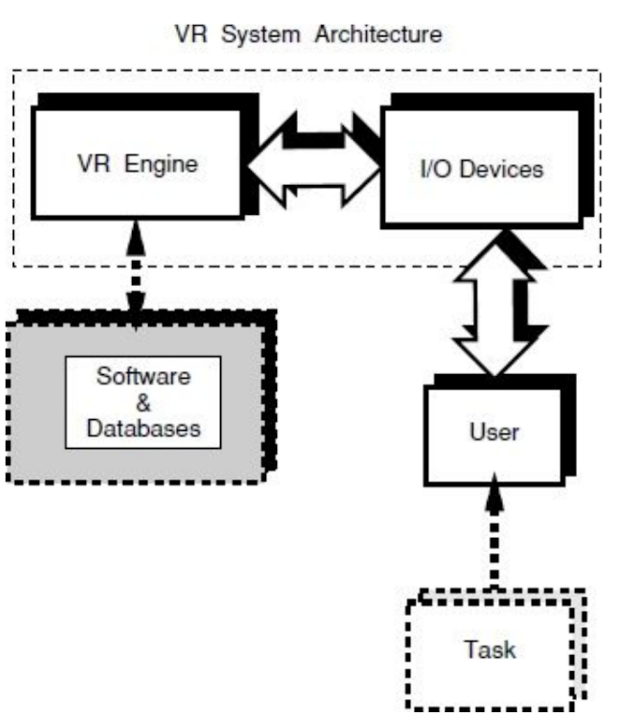
\includegraphics[width=0.5\textwidth]{IMG/VRarq.PNG}
    \caption{Arquitectura propuesta por \cite{burdea2003virtual} }
   \label{fig:RVarq}
\end{figure}
Según \emph{Burdea y Coiffet}\cite{burdea2003virtual}, un sistema de \ac{RV} se puede dividir en cinco componentes \new{tal y} como se puede observar en la figura \ref{fig:RVarq}. En ella se puede observar las distintas interacciones que se producen entre \new{los} componentes. De manera separada, estos componentes pueden existir independientemente pero es la relación \new{que existe} entre ellos, la que componen un sistema \new{de} \ac{RV}. A continuación, se describirá cada uno de ellos:
\begin{itemize}
    \item Motor de \ac{RV}: Este componente se encarga de realizar los cálculos necesarios para simular la escena virtual. Para actualizar el estado de la escena virtual, es necesario que \new{se} consulte las bases de datos y software incluidos en el sistema y actuará según la entrada recibida a través de los dispositivos realizada por los usuarios. El motor generará y mostrará el nuevo estado de la escena a través de los dispositivos de salida (que pueden incluir más de un canal sensorial). Además, es preciso asegurar una tasa interactiva al realizar estos cálculos. El término motor de RV no se puede asociar a un computador, sino que se tiene que tratar como una abstracción ya que puede tener múltiples configuraciones hardware como puede ser un único computador o un sistema distribuido conectado por red.
    \item Dispositivos de \ac{E/S}: Este componente se basa en todos los dispositivos que utilice el usuario en su interacción con el sistema. Es imprescindible en un sistema \new{de} \ac{RV} \new{se} permita la interacción del usuario. Los dispositivos de entrada se encargan de recoger las acciones que realiza el usuario, mientras que los dispositivos de salida muestran la respuesta de la escena virtual a través de los distintos canales sensoriales. Estos dispositivos son muy numerosos y diversos actualmente.
    \item Componentes software y base de datos: Este módulo contiene todas las especificaciones y descripciones que caracterizan el sistema. Aquí se incluyen la escena virtual y su organización que es consultada por el motor de \ac{RV} análogamente a lo que correspondería como una base de datos, donde se consulta y se recoge la información necesaria para la simulación. Además, aquí se incluyen, por ejemplo, las aplicaciones que se diseñan con el objetivo de guiar y facilitar el entrenamiento al dirigir la simulación según la interacción del sistema y el usuario.
    \item Usuario: Es natural que los sistemas se diseñen con el objetivo de que una persona \del{interaccionará} \new{interaccione} con ellos. Esta comunicación se realizará a través de los dispositivos de \ac{E/S}. 
    \item Tareas: Por último, son las tareas, objetivos e instrucciones que se le dan al usuario cuando va a utilizar el sistema \new{de} \ac{RV} que le dan significado y utilidad al simulador. Es lo que le diferencia de ser un computador con periféricos conectados de una plataforma de entrenamiento para pilotos o médicos. 
    
\end{itemize}

Esta definición de arquitectura será utilizada en el capítulo \ref{cap:rasim} como apoyo para explicar el simulador \ac{RASim} y sus diferentes componentes. A su vez, también puede ayudar al lector a hacerse una idea de como se han construidos los simuladores que se presentarán en las siguientes secciones.

\subsection{Simuladores para formación médica}
\label{art:medicalsim}

En los últimos años, los simuladores médicos de realidad virtual están tomando una gran importancia en el currículum de los estudiantes, como pueden ser los cirujanos y otras especialidades \cite{PATEL2017266.e7}. Se puede observar un incremento de su presencia para el entrenamiento de jóvenes especialistas tanto en hospitales como universidades. Estas herramientas proporcionan al usuario un método seguro y efectivo de entrenamiento, siendo capaces de usarlo tantas veces como sea posible. 

Aun con la introducción de los simuladores, el entrenamiento médico todavía se basa en una variedad de técnicas que permite al médico adquirir las destrezas necesarias antes de poder enfrentarse a escenarios reales de manera autónoma. Una forma segura de entrenamiento es la utilización de \emph{fantomas}\cite{phantomra}. En la figura \ref{fig:phantom} se puede ver un maniquí \emph{Blue Phantom™}\cite{BluePH} para la práctica de ultrasonografía.

\begin{figure}[h]
   \centering
    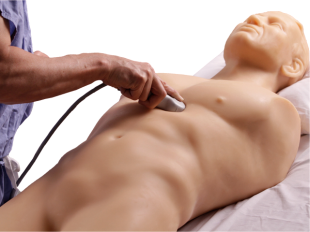
\includegraphics[width=0.5\textwidth]{IMG/fast_trauma.jpg}
    \caption{Maniquí realista para el entrenamiento de ultrasonografía  \emph{Blue Phantom™}\cite{BluePH} }
   \label{fig:phantom}
\end{figure}

Estos \emph{fantomas}\footnote{castellanización del término inglés Phantom} son modelos anatómicos hechos con materiales sintéticos intentando replicar el cuerpo humano fielmente y sus propiedades. En ocasiones, tienen incorporados una serie de sensores que permiten recogida de métricas. A pesar de que son muy populares, tienen una serie de inconvenientes: no son baratos, y suelen ser creados específicamente para una zona anatómica concreta, no siendo posible usarlos en otras circunstancias para lo que fueron creados. Además, si en determinadas ocasiones, el usuario tiene que manipularlos como puede ser hacer una incisión o inyección en el \emph{fantoma}, el modelo sufre desgaste con el tiempo.

Otra forma de entrenamiento es la utilización de cadáveres\cite{Tsui2007}, que permiten una anatomía real muy alejada de los muñecos. En este caso, conseguir diferentes variaciones anatómicas es completamente viable y el mismo cadáver puede servir para entrenamientos de diferentes procedimientos. Aun así, los inconvenientes que presentan son bastante evidentes. Mantener un cadáver en buenas condiciones o que los motivos del fallecimiento perjudiquen al estado del mismo, además de ciertos problemas éticos como puede ser el uso de cadáveres procedentes de condenados a pena de muerte (Visible Human Project \cite{ackerman1998visible}). Introducir sensores o algún tipo de dispositivo que permitan evaluar el rendimiento tampoco es sencillo. Finalmente, los tejidos de un cadáver no muestran el mismo comportamiento mecánico que un paciente, y puede inducir sesgos en el entrenamiento del médico debido a que los músculos se vuelven más rígidos después del fallecimiento.


La última forma de entrenamiento es, el entrenamiento sobre pacientes reales donde el estudiante realiza el procedimiento supervisado y guiado por su tutor. Aunque es el entrenamiento más realista, obviamente incluye una serie de riesgos y situaciones no controladas que pueden ser peligrosas para el paciente.


A diferencia de los métodos anteriormente citados, los simuladores de realidad virtual permiten un entrenamiento más barato y rápido donde los estudiantes pueden mejorar sus habilidades\del{.}\new{:} Mejoras en el rendimiento, nuevos dispositivos de \ac{E/S} y el desarrollo de nuevas técnicas de simulación física\del{,} permiten una transferencia efectiva de habilidades del mundo virtual al mundo real. Habitualmente los simuladores  son específicos de cada procedimiento médico donde podemos encontrar un simulador de cirugía ortopédica \cite{cecil2017advanced}, o por ejemplo un simulador de cirugía cardiovascular \cite{korzeniowski2018vcsim3}. Incluso, podemos incluir diferentes tipos de simulación, donde \cite{villard2014interventional} es un simulador de radiología intervencional \new{el cual} \del{donde} además de entrenar la habilidad manual, es necesario aprender como guiar la aguja a través de imagen de rayos X.

Pero además, la nueva generación de simuladores no solo se centran en mejorar la calidad de la simulación, sino que también quieren permitir el entrenamiento con datos de pacientes reales\cite{Willaert2012,  Votta2013}. 






\subsection{Diagnóstico por imagen médica}
\label{art:xraysim}

Dentro de la medicina, hay multitud de técnicas y procesos que generan imágenes médicas del paciente que se utilizan para el \del{diagnosis} \new{diagnóstico} de enfermedades, afección o dolencia. Existen multitud de técnicas anteriormente mencionadas (\ac{US}, \ac{TC}, \ac{IRM}, etc.) según la tecnología en las que están basadas. Esto caracteriza su utilización dependiendo de que tejidos o que imágenes se generan del cuerpo del paciente. 

En esta tesis, solo se centrará en el diagnóstico por imagen con rayos X. Esta especialidad médica se centra en la generación e interpretación de imágenes que se consiguen al exponer la anatomía objetivo a una radiación electromagnética que será recogido por un detector. Antiguamente, se proyectaba sobre películas fotográficas especialmente preparadas para la fuente emisora. Sin embargo, actualmente la mayoría de imágenes son almacenadas digitalmente gracias a un detector que permiten guardarlas directamente en un computador.

Se denomina proyecciones radiológicas al procedimiento de situar tanto al paciente como el equipo de radiología para conseguir una imagen de una parte concreta de la anatomía del paciente. Esta técnica define una proyección por cada parte del cuerpo a diagnosticar, y requiere por cada procedimiento una postura del paciente y configuración del equipo de radiografía concreto.

Según el libro \cite{manualpractico}, el procedimiento habitual que se debe seguir se resume en los siguientes pasos:
\begin{enumerate}
    \item Elección de \emph{bucky}: Elemento para reducir la radiación no perpendicular al detector. Este filtro suele utilizarse siempre, excepto en condiciones de emergencia o limitaciones físicas.
    \item Tamaño del chasis y orientación: Colocar el detector de la manera que permita cubrir la anatomía a estudiar.
    \item Posición del paciente: Teniendo en cuenta las limitaciones del paciente, se debe posicionar al paciente de pie, sentado o decúbito.
    \item Posición de la región anatómica: 
    Se colocará al paciente de tal forma que la región objeto de estudio se situé correctamente centrado respecto al chasis.
    \item Distancia foco película: Se sitúa el emisor de rayos X a la distancia adecuada para la proyección.
    \item Angulación: Existen algunas proyecciones donde el chasis se inclina para evitar superposición de estructuras.
    \item Centraje: Se centra la proyección de los rayos X en el centro de la región anatómica a estudiar, para lo que es fundamental el conocimiento de la anatomía.
    \item Colimación: Se reduce la apertura de la radiación para reducir la exposición del paciente.
    \item Técnica aproximada: Se configurará la potencia del equipo de radiología con el objetivo de reducir los niveles de exposición a lo mínimo posible, manteniendo la calidad diagnóstica (principio ALARA del inglés \emph{As Low AS Reasonably Achievable}\cite{manualpractico}). 
    \item Indicaciones al paciente: Ordenes al paciente en el momento de tomar la imagen.
\end{enumerate}
Al igual que se indica en el propio libro, esta metodología, y en concreto los valores de potencia de los emisores de radiación, no es estándar y es susceptible de variaciones, dependiendo generalmente del centro de trabajo, profesionales, escuelas, rendimiento y antigüedad de los equipos, etc. 

En cuanto a la enseñanza de las proyecciones radiológicas, la forma más común de aprender diagnóstico por imagen son los archivos educativos. Son recopilaciones de imágenes médicas de pacientes reales acompañados normalmente del historial del paciente. En estos archivos, los estudiantes pueden buscar a través de la gran cantidad de casos bien documentados. Es habitual que, cada universidad, hospital o facultad, tengan sus propios repositorios. Adicionalmente, existen libros donde se pueden consultar recomendaciones y guías \cite{carver2012medical,manualpractico}.
En la última década, cada vez más se publican estos recursos de manera \emph{online} donde cualquier radiólogo pueda consultar una enorme base de datos de imágenes de cualquier parte de la anatomía humana \cite{deshpande2017integrated}. 

Actualmente, la educación se ha visto beneficiada por la incorporación de los teléfonos inteligentes en este ámbito. Algunas instituciones han creado aplicaciones donde los estudiantes pueden revisar e investigar los casos almacenados, realizar cuestionarios y mejorar el aprendizaje como es el caso de la aplicación \emph{UBC Radiology} \cite{Spouge2017}. Estos recursos se encuentran muy presentes en el aprendizaje de los radiólogos noveles.

Tanto estos recursos como los archivos educativos mantienen el mismo problema: las imágenes registradas son estáticas, y la mayoría de estas imágenes corresponden a imágenes que se presuponen que son correctas y no muestran ningún tipo de fallo. Esto es completamente entendible, ya que al hacer este tipo de recursos se seleccionan aquellas imágenes que sean beneficiosas para el estudiante. Además, en estos recursos, ninguna imagen pertenece al mismo paciente por razones de seguridad. No es posible ver la misma anatomía u otras partes del mismo sujeto, que puedan mostrar diferentes situaciones al estudiante. Aun así, posicionar bien al paciente mientras se realiza el diagnóstico por imagen es algo imprescindible y algo necesario que el estudiante domine. 

\new{Por otra parte, las} Mejoras en el rendimiento de los computadores permiten crear nuevos simuladores que mejoran y reducen el tiempo de aprendizaje de los estudiantes. Un caso remarcable es el  ProjectionVR$^{TM}$ \cite{shanahan2016student}. Este simulador trata de introducir al usuario dentro de un entorno realista 3D que replica una sala de radiología con el objetivo de simular el procedimiento completo. Con datos de pacientes reales digitalizados, el simulador replica un entorno de aprendizaje sin el consecuente riesgo de radiación que significaría exponer a los estudiantes o los pacientes. Aunque provee una cantidad amplia de datos médicos, los datos que contienen son estáticos y los usuarios no pueden variarlos o modificarlos en el simulador. También es notable mencionar la herramienta \emph{medspace.VR} \cite{medspace}. Este simulador proporciona un escenario virtual muy realista que ayuda al usuario a practicar el procedimiento de manera sistemática. Aun así, solo presenta un paciente virtual que únicamente contiene los tejidos de la piel y los huesos, sin ningún otro modelo interno que pueda ayudar a la correcta identificación de la anatomía del paciente.

%https://www.bluephantom.com/product/Sciatic-Nerve-Regional-Anesthesia-Ultrasound-Training-Model.aspx?cid=428


\subsection{Anestesia regional}

Como se ha introducido anteriormente, existen multitud de simuladores dependiendo del procedimiento médico que se pretende simular. En cuanto a la especialidad de anestesiología, la anestesia espinal y la epidural son los dos ejemplos más frecuentes dentro de la \ac{RA} y podemos encontrar simuladores específicos \cite{broom2018evaluation}. Sin embargo, la búsqueda de un simulador de \ac{RA} genérico es más complicada. Energid Technologies ha desarrollado  un simulador en un contrato con el Ejército de Estados Unidos, pero no ha sido comercializado al público \cite{lim2008simulation}.

Otro simulador, en este caso comercial, llamado SAILOR es distribuido acompañado de un atlas multimedia de los bloqueos de nervios. Este simulador presenta solo un único modelo de paciente, y su interacción es exclusivamente con el ratón sin ninguna tipo de deformación del tejido\cite{Bibin}. 

En un estudio previo al proyecto \ac{RASimAs}, se demostró la aceptación que tendría un simulador para la \ac{RA}. Todos los participantes se mostraron muy receptivos con el trabajo realizado pero, sin embargo, se pudo constatar la escasez de nervios para bloquear, la pobre simulación de los ultrasonidos y la ausencia de respuesta háptica \cite{Grottke2009594}.

%https://www.gtsimulators.com/Full-Body-X-Ray-Phantom-with-Real-Human-Skeleton-p/ez7200.htm